    \subsection*{Example: Linear Regression}
    
        Let's go through some \textbf{examples}. We mentioned in the \textbf{beginning} of this chapter that our neuron could be most of the simple \textbf{models} we've worked with.
        
        So, let's give that a go: we'll start by doing \textbf{linear regression}.
        
        \begin{equation*}
            h(x) = \theta^T x + \theta_0
        \end{equation*}
        
        This model is exclusively \textbf{linear}: we just have to replace $\theta$ with $w$.
        
        \begin{equation*}
            \red{z}(x) = w^T x + w_0
        \end{equation*}
        
        So, our linear component is \textbf{done}: $(\theta, \theta_0) = (w, w_0)$.
        
        What about our \textbf{activation} function?
        
        Well, activation allows for \textbf{nonlinear} functions. But, we don't \textbf{want} to make it nonlinear. 
        
        In fact, we've already got what we \textbf{want}: we don't want the \textbf{activation} to do anything at \textbf{all}.
        
        So, we'll use \textbf{this} function:\\
        
        \begin{concept}
            The \vocab{identity function} $f(z)$ is a function that has no \gren{effect} on your \purp{input}.
            
            \begin{equation*}
                f(\red{z}) = \red{z}
            \end{equation*}
            
            By "having no effect", we mean that the input is \purp{unchanged}: this is true even if your input is \gren{another function}:
            
            \begin{equation}
                f(g(x)) = g(x)
            \end{equation}
        \end{concept}
        
            \note{We call it the "identity" because the input's identity is unchanged!}
        
        So, the \textbf{identity} function is our activation function: it keeps our \textbf{linearity}.\\
        
        \begin{concept}
            \vocab{Linear Regression} can be represented with a \gren{single neuron} where
            
            \begin{itemize}
                \item We keep our \purp{linear component}, but set $(\theta, \theta_0) = (w, w_0)$.
                
                \begin{equation*}
                    \red{z}(x) = w^Tx+w_0
                \end{equation*}
                
                \item Our \purp{activation function} is the \gren{identity} function, 
                
                \begin{equation*}
                    f(\red{z}) = \red{z}
                \end{equation*}
                
                \item Our \purp{loss function} is \gren{quadratic loss}.
                
                \begin{equation*}
                    \loss(\pur{a},y) = (\pur{a}-y)^2
                \end{equation*}
                
            \end{itemize}
        \end{concept}
        
        \begin{figure}[H]
            \centering
            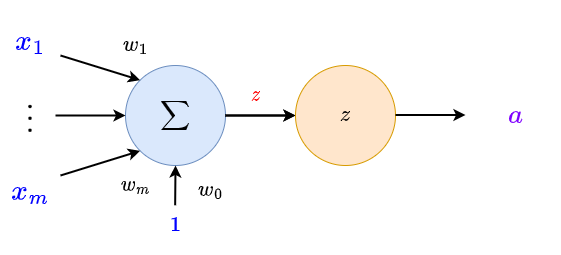
\includegraphics[width=100mm,scale=0.4]{images/nn_images/linear_reg.png}
        \end{figure}
    
    \subsection*{Example: Linear Logistic Classifiers}
    
        Now, we do the same for LLCs: it's already broken up into \textbf{two} parts in our \textbf{classification} chapter.
        
        First, the \textbf{linear} component. This is the same as linear regression:
        
        \begin{equation}
            \red{z} = 
            \theta^T x + \theta_0
        \end{equation}
        
        And then, the \textbf{logistic} component:
        
        \begin{equation}
            \sigma(\red{z}) = \frac{1}{1+e^{-\red{z}}}
        \end{equation}
        
        This second part is \textbf{nonlinear}: its our \textbf{activation} function!\\
        
        \begin{concept}
            A \vocab{Linear Logistic Classifier} can be represented with a \gren{single neuron} where
            
            \begin{itemize}
                \item We keep our \purp{linear component}, but set $(\theta, \theta_0) = (w, w_0)$.
                
                \begin{equation*}
                    \red{z}(x) = w^Tx+w_0
                \end{equation*}
                
                \item Our \purp{activation function} is the \gren{sigmoid} function, 
                
                \begin{equation*}
                    f(\red{z}) = \sigma(\red{z}) = \frac{1}{1+e^{-\red{z}}}
                \end{equation*}
                
                \item Our \purp{loss function} is \gren{negative-log likelihood} (NLL)
                
                \begin{equation*}
                    \loss_{nll}
                    (\pur{a} ,\quad \byi)
                    =
                    -
                    \Bigg(
                        \byi \log{\pur{a}}
                        +
                        \left( 1 - \byi \right)
                        \log
                        \left( 1-\pur{a} \right) 
                    \Bigg)
                \end{equation*}
            
            \end{itemize}
        \end{concept}
        
        \begin{figure}[H]
            \centering
            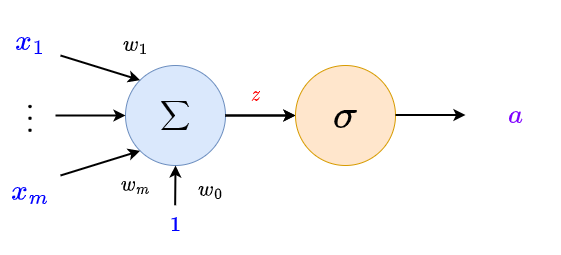
\includegraphics[width=100mm,scale=0.4]{images/nn_images/llc_unit.png}
        \end{figure}
        